\documentclass[12pt]{report}
\usepackage{balance}			                    % proper column balancing 
\usepackage{cite}			                        % well-formed numeric citations
\usepackage{epsfig}			                        % add support for `EPS' figures
\usepackage{epstopdf}			                    % automatic `EPS' to `PDF' conversion
\usepackage[T1]{fontenc}		                    % enable `Type 1' fonts
\usepackage[pagebackref = false, pdftex]{hyperref}	% add support for hypertext marks
\usepackage{graphicx}			                    % add support for graphics
\usepackage{listings}			                    % add support for source code listings
\usepackage{mathptmx}			                    % use `Times' as the default font
\usepackage{subfigure}			                    % add support for `subfloats'
\usepackage{tikz}			                        % add support for custom graphics
\usetikzlibrary{calc} 
\usepackage{verbatim}	                            % better `verbatim'
\usepackage{xcolor}			                        % add support for color names
\usepackage{xspace}			                        % proper macro spacing
\usepackage{mdframed}
\usepackage{geometry}
\usepackage{minted}
\setminted{breaklines}
\usepackage{wrapfig}

\usepackage{etoc}

\geometry{
    a4paper,
    left = 3.5cm,
    top = 2.5cm,
    right = 2.5cm,
    bottom = 3.0cm
}

% title, keywords
\def\ptitle{Exploring Swift as a Serverless Language on OpenWhisk}
\def\pkeywords{swift, serverless, openwhisk, faas}

% comment out the following line to disable comments in text
% \newcommand{\commentsenabled}{X}
% comment commands
\ifdefined\commentsenabled
\newcommand{\el}[1]{\textbf{\color[rgb]{1,0,0} elathan: #1}}
\newcommand{\pw}[2]{\textbf{\color[rgb]{0,0,1} yourhandle: #1}}
\else
\newcommand{\el}[1]{}
\newcommand{\pw}[2]{}
\fi

% listings setup
\lstset{
	backgroundcolor	= \color{white},
	basicstyle	= \scriptsize,
	breaklines	= true,
	captionpos	= b,
	commentstyle	= \color{gray}\ttfamily,
	frame		= lines, 
	language	= C++, 
	numbers		= left,
	tabsize		= 2,
	xleftmargin	= 6pt,
}

% hyperref setup
\hypersetup{
	unicode,
	citecolor	= black,
	colorlinks	= true,
	filecolor	= black,
	linkcolor	= black,
	pagebackref	= true,
	pdfkeywords	= {\pkeywords},
	pdftitle	= {\ptitle},
	urlcolor	= black,
} 

% checkmark
\def\checkmark{\tikz\fill[scale=0.4](0,.35) -- (.25,0) -- (1,.7) -- (.25,.15) -- cycle;} 

% hacks
\newenvironment{code}{\small\verbatim}{\endverbatim\normalsize}
\newcommand{\note}[1]{\noindent\textbf{\color{red}[#1]}}
\newcommand{\commentout}[1]{}

% custom macros
\newcommand{\ie}{\emph{i.e.,}\xspace}
\newcommand{\eg}{\emph{e.g.,}\xspace}
\newcommand{\etc}{\emph{etc.}\xspace}

\linespread{1.25} 


\begin{document}
\begin{titlepage}
\begin{center}
\vspace*{1cm}

Thesis Dissertation

\vspace*{2cm}
\begin{center}
\Large{\textbf{\MakeUppercase{\ptitle{}}}}
\end{center}

\vspace*{2cm}

\large{\textbf{Andreas Loizides}}

\vspace*{1cm}
\Large{\textbf{\MakeUppercase{University of Cyprus}}}

\vspace*{2cm}


\includegraphics[width=0.2\textwidth]{media/ucy-logo.png}

\vspace*{2cm}

\Large{\textbf{\MakeUppercase{Computer Science Department}}}

\vspace*{4cm}

\normalsize{May 2023}
\begin{tikzpicture}[remember picture, overlay]
  \draw[line width = 1pt] ($(current page.north west) + (1in,-1in)$) rectangle ($(current page.south east) + (-1in,1in)$);
\end{tikzpicture}
\end{center}
\end{titlepage}

\begin{titlepage}

\begin{center}
\LARGE{\textbf{\MakeUppercase{University of Cyprus}}}

\Large{\textbf{\MakeUppercase{Computer Science Department}}}

\vspace*{6cm}

\large{\textbf{\ptitle{}}}

\vspace*{0.5cm}

\large{\textbf{Andreas Loizides}}

\vspace*{5cm}

\large{Supervisor}

\large{Dr. Haris Volos}

\vspace*{4cm}

Thesis submitted in partial fulfilment of the requirements for the award of degree of Bachelor in Computer Science at University of Cyprus

\vspace*{1cm}

May 2023
\end{center}

\end{titlepage}

\chapter*{Acknowledgements}
\addcontentsline{toc}{chapter}{Acknowledgements}

I would like to express my profound gratitude to a number of people whose support and contributions were invaluable throughout the course of this thesis.

First and foremost, I would like to thank my supervisor and mentor, Dr. Haris Volos, for his unwavering guidance and continuous support. Whenever issues arose, Dr. Volos was always ready to thoroughly evaluate the problem, imparting not only his expert knowledge but also a sense of shared purpose and curiosity. His dedication to my research gave me the confidence and motivation to navigate the complex challenges that arose during this thesis. It truly felt like we shared the same research goals and the drive to satisfy curiosity which is crucial in a research context. His care and attention were instrumental in enabling me to reach my research goals.

I am deeply grateful to my university for granting me access to the CloudLab's infrastructure. This access was not just a privilege but a necessity. The comprehensive results and the eventual completion of this thesis would not have been possible without it. It provided a robust platform to explore Swift as a serverless language on OpenWhisk, contributing significantly to the outcomes of my research.

Lastly, but by no means least, I would like to extend my heartfelt thanks to my parents. Their unconditional faith in my abilities and their financial support provided a stable foundation for my academic journey. It allowed me to comfortably pursue my interests and devote my energy to my research. Their sacrifices and belief in my vision were a beacon of light that guided me through the most challenging phases of this thesis.

To all of you, thank you. This accomplishment would not have been possible without your collective support and belief.



\newpage

\chapter*{Summary}

This thesis delves into the potential of Swift in the rapidly growing field of serverless computing. Serverless computing has gained significant attention due to its scalability and cost-effectiveness, making the choice of programming language a crucial factor in this context.

Swift, a language renowned for its popularity on Apple platforms, is known for its speed, safety, and reliability. Despite its widespread use in the Apple ecosystem, Swift's potential as a serverless language remains largely unexplored. This thesis aims to bridge this gap, driven by Swift's promise of speed and safety.

The methodology for evaluating Swift's capabilities as a serverless language involves a two-pronged approach. Initially, a qualitative comparison is conducted with popular serverless languages to investigate potential performance benefits Swift might provide. Subsequently, Swift's capabilities are evaluated through a case study, comparing a serverless to a monolithic implementation of a synchronization system.

The key findings from the research indicate that while Swift holds promise, its lack of community support and unstable Linux support with various functionalities missing, make it unsuitable for production use as a systems language, let alone serverless. Furthermore, the case study highlighted OpenWhisk's need to support intra-concurrency to fully utilize the hardware and achieve real concurrency in invoking actions.

In terms of benefits, Swift is enjoyable to write in and is a very expressive language. Most errors are caught at compile time, saving critical time and effort. Its seamless Copy-on-Write (CoW) support has the potential to greatly benefit memory and performance-critical environments, such as serverless. However, the limitations, particularly the lack of community support and ambiguity in many features in regards to their Linux support, pose significant challenges.

In conclusion, this thesis provides a comprehensive exploration of Swift as a serverless language, contributing to the ongoing discourse in this area and highlighting areas for further research.



\tableofcontents
\listoffigures
%\listoftables

% outline
\chapter{Introduction}
\etocsettocstyle{\rule{\textwidth}{1pt}}{\rule{\textwidth}{1pt}} % style for toc
\localtableofcontents
\section{Background}

The landscape of computing has witnessed a paradigm shift in recent years, with the emergence of serverless computing. Serverless computing enables developers to focus on writing their application's code without worrying about underlying infrastructure management, provisioning, and scaling. As a result, serverless computing has gained popularity as a cost-effective and scalable alternative to traditional web and application development practices. Some of the many advantages of serverless computing include auto-scaling, elimination of idle server costs, pay-per-use pricing, and seamless scaling to handle fluctuating workloads.

In the realm of serverless computing, one's choice of a programming language is crucial. It affects not only the performance but also the ease of development and maintenance of serverless applications. The focus of this thesis is the Swift programming language, which has demonstrated its potential for speed, safety, and reliability, particularly in Apple platforms.

\section{Swift in Serverless Computing}

Swift is a statically typed, general-purpose, multi-paradigm programming language developed by Apple Inc. for iOS, macOS, watchOS, and other platforms. Since its release in 2014, Swift has gained significant popularity and achieved acclaim for its efficiency, safety, and ease of use. The Swift programming language demonstrates potential as a viable serverless language due to its inherent speed, safety, and its compatibility with OpenWhisk, which is the selected environment for this study.

\section{Choice of Serverless Environment: OpenWhisk}

OpenWhisk is an event-driven, open-source serverless computing platform that supports a wide range of programming languages, including Swift, Python, Java, and Node.js. The reasons for selecting OpenWhisk as the environment for this study include its widespread adoption in serverless computing contexts, its flexibility, and its support for Swift as a first-class language. For the purpose of the comparative analysis in this thesis, we will examine the advantages and disadvantages of using Swift against other popular serverless computing languages such as Python, Java, and Node.js, all of which have established themselves in this domain.

\section{Case Study: Synchronization System in eCommerce}

A case study detailing a monolithic and serverless implementation of a synchronization system in the eCommerce industry will be presented in this thesis. The synchronization system serves a critical function in ensuring consistency and accuracy across online stores, as it aids in maintaining inventory, order management, and customer accounts up-to-date. This case study will help demonstrate Swift's viability as a serverless language in a real-world scenario and contribute to the broader discussion on the appropriateness of Swift for serverless computing.

\section{Research Questions}
With the background and context established, this thesis will attempt to answer the following research questions:

\subsection{Performance Comparison}
How does the performance of Swift in serverless computing compare to other languages, such as Python, Java, and Node.js? This involves examining any potential benefits Swift could provide over other languages in a serverless context, as well as any possible performance limitations or challenges it may present.

\subsection{Ease of Development}
To what degree is Swift an accessible and efficient language for developers in a serverless environment? This question will be addressed through evaluating the development experience of Swift compared to other serverless languages, investigating aspects such as language features, syntax, tooling, and libraries that impact the ease of development of serverless functions in Swift.

\section{Objective}

The overarching objective of this thesis is to provide a comprehensive analysis of Swift as a serverless language, examining its potential for performance and ease of development within the OpenWhisk environment. By conducting an in-depth comparison with other common serverless languages and illustrating Swift's applicability through a practical case study, this thesis aims to contribute valuable insights and perspectives, further advancing the understanding of Swift's role in serverless computing.

%\section{Thesis Structure}
%
%The structure of this thesis is as follows:
%\begin{itemize}
%    \item Chapter 2: A comprehensive review of serverless computing, its benefits, challenges, and related programming languages.
%    \item Chapter 3: An introduction to Swift, its language features, and a discussion of its suitability for serverless computing.
%    \item Chapter 4: A detailed comparison of Swift with other popular languages for serverless computing: Python, Java, and Node.js, guided by the research questions on performance and ease of development.
%    \item Chapter 5: An overview of the OpenWhisk environment, its key components, and a justification for its selection in this thesis.
%    \item Chapter 6: A presentation of the case study comparing monolithic and serverless implementations of a synchronization system in eCommerce.
%    \item Chapter 7: An analysis of the case study, discussing the benefits and drawbacks of using Swift in this context.
%    \item Chapter 8: Conclusion and future research directions.
%\end{itemize}
%\input{chapters/literature_review.tex}
%\chapter{Related Work}
\label{chap:relatedwork}

This chapter provides a brief review of the existing literature relevant to the use of Swift as a serverless language on OpenWhisk. 

\section{Introduction}
The concept of serverless computing has gained considerable attention in recent years. The promise of serverless is to simplify cloud programming by eliminating the need for developers to manage servers and allowing them to focus solely on their application logic. Jonas et al. \cite{Jonas:EECS-2019-3} provide a thorough overview of this paradigm, tracing its history from the early days of cloud computing to the present. They argue that serverless computing is the next step in the evolution of abstraction in computing, comparing it to the shift from assembly language to high-level programming languages. The authors also identify areas where serverless computing is pushing the boundaries, as well as the challenges and research opportunities that lie ahead. They predict that serverless computing will become a predominant model in the future of cloud computing.

\section{OpenWhisk}
OpenWhisk, an open-source serverless platform, has been the subject of numerous studies. Castro et al. \cite{castro2020openwhisk} provide an in-depth analysis of OpenWhisk's architecture and capabilities, offering valuable insights into its potential for hosting Swift-based serverless applications. This comprehensive study of OpenWhisk provides an essential foundation for understanding the possibilities and constraints of running Swift applications in a serverless environment.

\section{Serverless Computing and Languages}
The choice of programming language in serverless computing is an important aspect that has significant implications on the performance and efficiency of serverless applications. A study by \cite{implications-prog} investigates the impacts of programming language selection on the performance of serverless data processing pipelines. By implementing identical data processing pipelines in multiple languages (Java, Python, Go, and Node.js), the authors demonstrate that the performance of a pipeline can vary significantly based on the chosen language. Their study concludes that there is no one-size-fits-all language for serverless computing. Instead, they suggest that the fastest and most efficient pipeline could be achieved by adopting a hybrid approach, combining different languages to optimize various stages of the pipeline. This underlines the importance of careful language selection and performance profiling before deploying serverless applications, indicating that the choice of language can have substantial consequences on the overall performance and efficiency of serverless applications.

\section{Research Gaps}
Despite the wealth of knowledge available on serverless computing and OpenWhisk, there is a noticeable gap in the literature when it comes to using Swift as a serverless language. Few studies have specifically explored the performance, advantages, and challenges of using Swift in a serverless context, particularly on the OpenWhisk platform. This thesis aims to address this gap by providing an in-depth exploration of Swift as a serverless language on OpenWhisk. The goal is to gain a deeper understanding of the potential of Swift in this context and to contribute to the broader discourse on serverless computing and language choice.


\chapter{Updating the Swift Runtime for OpenWhisk}
\etocsettocstyle{\rule{\textwidth}{1pt}}{\rule{\textwidth}{1pt}} % style for toc
\localtableofcontents

\section{Introduction to the need for updating the Swift runtime}
\subsection{Runtimes in OpenWhisk}

In serverless platforms like OpenWhisk, the unit of execution for functions is a container that runs the user's code. These containers are based on pre-configured runtimes, which provide the necessary environment and dependencies to run code written in specific languages. OpenWhisk supports several languages and runtimes out-of-the-box, but it also allows custom runtimes for users who require tighter integration with their specific language or environment needs.

An OpenWhisk runtime follows specific interface requirements and has to adhere to the platform specifications. A runtime should generally perform the following tasks: initialization, activation, and logging. Initialization prepares the runtime container for execution based on the user's code; activation manages the input parameters, runs the function, and returns the function result; and logging captures all the output generated during activation.

\subsection{ActionLoop Proxy}

To include a custom language runtime in OpenWhisk, the runtime must follow certain platform requirements and best practices. It should be implemented in a separate repository to ensure its management lifecycle remains independent of the OpenWhisk platform. Additionally, the runtime must be both introduced into the runtime manifest and included in the Swagger file, accompanied by relevant documentation files describing its usage.

Testing the newly implemented runtime is crucial for ensuring that it is reliable and adheres to the OpenWhisk project's standards. The new runtime repository should include a series of test actions that conform to the Canonical runtime repository layout and successfully pass multiple test suites, including Action Interface tests and Runtime proxy tests.

In this chapter, we will discuss the need for updating the Swift runtime to support the latest version (5.8) and the benefits that the newer language features can bring to serverless computing on the OpenWhisk platform. We will then detail the challenges encountered during the updating process, describing the steps taken to update the Swift runtime, and verifying the updated runtime functionality that can benefit future researchers exploring serverless computing with Swift.

\section{Overview of the officially supported Swift runtime in OpenWhisk}
Apache OpenWhisk supports a variety of programming languages for writing actions, through the use of specific runtimes. As per the official documentation, the following runtimes are currently supported 
~\cite{openwhisk2023}:

\begin{itemize}
\item .Net: OpenWhisk runtime for .Net Core 2.2.
\item Go: OpenWhisk runtime for Go.
\item Java: OpenWhisk runtime for Java 8 (OpenJDK 8, JVM OpenJ9).
\item JavaScript: OpenWhisk runtime for Node.js v10, v12, and v14.
\item PHP: OpenWhisk runtime for PHP 8.0, 7.4, and 7.3.
\item Python: OpenWhisk runtime for Python 2.7, 3, and a 3 runtime variant for AI/ML (including packages for Tensorflow and PyTorch).
\item Ruby: OpenWhisk runtime for Ruby 2.5.
\item Swift: OpenWhisk runtime for Swift 3.1.1, 4.1, and 4.2.
\end{itemize}

These runtimes are officially released by the Apache OpenWhisk project and made available on the OpenWhisk Downloads page.

\section{Benefits of newer Swift features for serverless computing}
% Content here, such as async/await

\section{Challenges faced while updating the runtime}
% General challenges content here

\subsection{Understanding the current runtime architecture}
% Content about understanding the current architecture

\subsection{Implementing support for the latest Swift version (5.8)}
% Content about implementing support for Swift 5.8

\section{Steps to update the Swift runtime in OpenWhisk}
% General steps content here

\subsection{Description of the process and tools required}
% Content about the process and required tools

\subsection{Code snippets and configuration changes for updating the runtime}
% Content about code snippets and configuration changes, use listings or any other preferred package for code snippets

\section{Verifying the updated runtime functionality}
% General content about verifying the updated runtime

\subsection{Testing and validating the new runtime with the synchronization system case study}
% Content about testing and validation with the case study

\section{Potential benefits and applications of the updated runtime for future researchers}
% Content about potential benefits and applications

\section{Possible further improvements or updates to the runtime}
% Content about possible improvements or updates to the runtime

%\input{chapters/research_methodology.tex}
\chapter{Performance Overview}
\etocsettocstyle{\rule{\textwidth}{1pt}}{\rule{\textwidth}{1pt}} % style for toc
\localtableofcontents
In this chapter, we examine some qualities of Swift that could give it a performance edge over other languages. What are those qualities? Do other serverless languages match them with anything similar? We aim to answer those questions.
\section{Value Types vs Reference Types and Copy-On-Write}
First, we have to understand the differentiation of value and reference types.
In programming languages, value types and reference types represent two ways to handle data. Understanding the difference between them and their performance implications is crucial to making informed decisions when choosing a language for serverless applications. Swift not only distinguishes between value and reference types, but also employs Copy-On-Write optimization for most of its value types, including collections such as Arrays, Dictionaries, and Sets.
This differentiation allows Swift to provide "free" CoW for Value types. That means a more efficient use of memory, which is more than crucial in memory-constrained contexts such as serverless.

\subsection{Value Types}

Value types are types for which the value is stored directly in the memory. When a value type is assigned or passed to a function, a separate copy of the value is created. The main benefit of value types is that they are generally more efficient in terms of memory usage and can result in more predictable performance. This is because allocation happens in the stack, which tends to be much faster than heap allocation, which is what happens for reference types. In Swift, the distinction between value and reference types is handled through structs (value types) and classes (reference types).

\subsection{Reference Types}

Reference types represent data where the memory location (or reference) is stored, rather than the data itself. When a reference type is assigned or passed to a function, the reference (memory address) is copied, not the actual data. This means that different variables can point to the same data, potentially leading to unexpected behavior if the data is modified.

\subsection{Copy-On-Write (CoW)}

Swift uses Copy-On-Write (CoW) for most of its value types, including collections such as Arrays, Dictionaries, and Sets. Collections whose Element type is also a value type essentially leverage CoW for free. CoW is an optimization strategy where the copying of a value type is delayed until it's necessary, i.e., when the value needs to be modified.

This approach has several performance benefits when compared to simply copying the data every time:

\begin{itemize}
  \item Sharing the same data among multiple instances of a collection is more memory efficient, as multiple copies of the same data are not required.
  \item When a value is not modified, the overhead of data copying is eliminated, resulting in improved performance.
  \item Copying is performed only when modifications are made, avoiding unnecessary data duplication.
\end{itemize}

\subsection{Performance Benefits}

The distinction between value and reference types, as well as Swift's usage of CoW, has several implications for performance:

\begin{itemize}
  \item Value types with CoW can lead to more predictable performance, as the compiler can make better optimization decisions when it knows that data cannot be shared or modified externally. Furthermore, the actual data copying is delayed until it's necessary.
  \item Copying value types can be faster, as the memory layout is more predictable and can often be associated with better cache utilization.
  \item Avoiding the overhead of managing memory references for reference types can result in performance improvements, as fewer indirections are needed for memory access.
\end{itemize}
For example, suppose in a backtracking algorithm, we execute a function on some data. The function may or may not modify it. Suppose we pass a copy of this data to the function, in order to later decide which one of the two to keep. If the one produced by the function is not desired, we "backtrack" to the previous version. In other languages, this copy of the data is guaranteed, even though the function may not modify it at all. In Swift, no copying takes place unless the function actually modifies it.

In summary, the distinction between value and reference types in a language like Swift, combined with the use of Copy-On-Write optimizations, provides developers with fine-grained control over memory handling and potentially leads to better performance when compared to languages that do not offer such a distinction. These aspects make Swift an attractive choice for serverless applications where performance is critical.


\section{Qualitive Comparison with Go, Java, Javascript, and Python}
Is the distinction between value types and reference types achievable in each language? Is any benefit from the distinction possible in each language? 
In this section, we will compare the distinction between reference and value types in Swift to Go, Python, Node.js (JavaScript), and Java. We will examine whether these languages offer a similar distinction, and if any benefits from the distinction are achievable in each language.

\subsection{Go}

Go supports both reference types and value types. In Go, structs are used as value types, while slices, maps, and channels are some examples of reference types.

\paragraph{Value types in Go:}
When a value type variable is assigned or passed to a function, a copy of the value is created. Consider the following example:

\begin{minted}{go}
package main

import "fmt"

type Point struct {
	X int
	Y int
}

func main() {
	p1 := Point{1, 2}
	p2 := p1
	p2.X = 3

	fmt.Println(p1) // Output: {1 2}
	fmt.Println(p2) // Output: {3 2}
}
\end{minted}

In this example, assigning \mintinline{go}{p1} to \mintinline{go}{p2} creates a separate copy of the value, hence changing \mintinline{go}{p2.X} does not affect \mintinline{go}{p1}.

\paragraph{Reference types in Go:}
While Go also has reference types, like slices, they behave differently than reference types in Swift. Here's an example using slices:

\begin{minted}{go}
package main

import "fmt"

func main() {
	s1 := []int{1, 2, 3}
	s2 := s1
	s2[0] = 9

	fmt.Println(s1) // Output: [9 2 3]
	fmt.Println(s2) // Output: [9 2 3]
}
\end{minted}

In this case, assigning \mintinline{go}{s1} to \mintinline{go}{s2} creates a reference to the same slice. Modifying \mintinline{go}{s2[0]} affects \mintinline{go}{s1} as well.

Although Go has value and reference types, it does not support Copy-On-Write (CoW) optimizations like Swift, limiting its potential for similar performance improvements.

\subsection{Python}

Python, being a dynamically typed language, does not explicitly provide separate value and reference types. However, the distinction can still be made between mutable and immutable objects, which relates to the concept of value and reference types.

\paragraph{Immutable objects:}
Immutable objects like tuples, strings, and frozensets behave similarly to value types:

\begin{minted}{python}
t1 = (1, 2)
t2 = t1
t2 += (3,)

print(t1)  # Output: (1, 2)
print(t2)  # Output: (1, 2, 3)
\end{minted}

In this example, updating \mintinline{python}{t2} by adding a new element does not affect \mintinline{python}{t1}.

\paragraph{Mutable objects:}
Mutable objects like lists, dictionaries, and sets behave more like reference types:

\begin{minted}{python}
l1 = [1, 2, 3]
l2 = l1
l2[0] = 9

print(l1)  # Output: [9, 2, 3]
print(l2)  # Output: [9, 2, 3]
\end{minted}

Here, assigning \mintinline{python}{l1} to \mintinline{python}{l2} creates a reference to the same list. Modifying \mintinline{python}{l2[0]} affects \mintinline{python}{l1} as well.

Python's performance characteristics are quite different from languages like Swift and Go. As Python does not have a built-in CoW mechanism and is generally slower due to its dynamic typing and interpreted nature, the benefits achievable from the distinction between value and reference types are comparatively limited.

\subsection{Node.js (JavaScript)}

JavaScript, the language used in Node.js, is also dynamically typed and principally uses reference types. All objects in JavaScript are reference types, including arrays and functions.

\paragraph{Reference types in JavaScript:}
When an object is assigned or passed to a function, it's the reference that is passed, not the actual data:

\begin{minted}{javascript}
let arr1 = [1, 2, 3];
let arr2 = arr1;
arr2[0] = 9;

console.log(arr1); // Output: [ 9, 2, 3 ]
console.log(arr2); // Output: [ 9, 2, 3 ]
\end{minted}

In this example, assigning \mintinline{javascript}{arr1} to \mintinline{javascript}{arr2} creates a reference to the same array. Modifying \mintinline{javascript}{arr2[0]} affects \mintinline{javascript}{arr1} as well.

\paragraph{Simulating value types in JavaScript:}
Although JavaScript does not have native value types, developers can simulate value-like behavior using techniques such as object cloning:

\begin{minted}{javascript}
function clone(obj) {
    return JSON.parse(JSON.stringify(obj));
}

let obj1 = { x: 1, y: 2 };
let obj2 = clone(obj1);
obj2.x = 3;

console.log(obj1); // Output: { x: 1, y: 2 }
console.log(obj2); // Output: { x: 3, y: 2 }
\end{minted}

Despite being able to simulate value types, the distinction between value and reference types in JavaScript is not as natural as it is in Swift. Furthermore, JavaScript lacks built-in CoW optimizations, limiting the performance benefits that can be derived from the distinction.

\subsection{Java}

Java, being an object-oriented language, primarily deals with reference types like classes and interfaces. Primitive types in Java, like \mintinline{java}{int}, \mintinline{java}{float}, and \mintinline{java}{boolean}, are value types.

\paragraph{Value types in Java:}
Java's primitive types are value types:

\begin{minted}{java}
int a = 1;
int b = a;
b = 3;

System.out.println(a); // Output: 1
System.out.println(b); // Output: 3
\end{minted}

In this case, assigning \mintinline{java}{a} to \mintinline{java}{b} creates a separate copy of the value. Changing the value of \mintinline{java}{b} does not affect \mintinline{java}{a}.

\paragraph{Reference types in Java:}
Java's objects behave as reference types:

\begin{minted}{java}
List<Integer> list1 = new ArrayList<>(Arrays.asList(1, 2, 3));
List<Integer> list2 = list1;
list2.set(0, 9);

System.out.println(list1); // Output: [9, 2, 3]
System.out.println(list2); // Output: [9, 2, 3]
\end{minted}

In this example, assigning \mintinline{java}{list1} to \mintinline{java}{list2} creates a reference to the same list. Modifying an element in \mintinline{java}{list2} affects \mintinline{java}{list1} as well.

Java has a more explicit distinction between value (primitive types) and reference types (objects). However, since Java does not have CoW optimizations like Swift, the potential performance benefits from such distinctions are more limited in comparison.

\section{Summary}

In summary, all five languages -- Swift, Go, Python, JavaScript (Node.js), and Java -- offer some degrees of distinction between value and reference types or related concepts (mutable/immutable objects). The distinction is often more explicit in statically-typed languages like Swift, Go, and Java, while dynamically-typed languages like Python and JavaScript handle the distinction via mutable/immutable objects or using programmer-provided methods for simulating value types.

However, the primary differentiator for Swift is its built-in Copy-On-Write (CoW) optimization for value types. This feature allows Swift to offer performance benefits for serverless applications that may not be as easily achievable in other languages under comparison. Performance improvements, both in terms of memory usage and execution time, can be derived from the proper understanding and application of the distinction between value and reference types, as well as making the most of the CoW optimization in Swift.

%\chapter{Startup Analysis of Serverless Languages on OpenWhisk}
\etocsettocstyle{\rule{\textwidth}{1pt}}{\rule{\textwidth}{1pt}} % style for toc
\localtableofcontents
\label{chap:cold_start_analysis}

\section{Introduction}
\label{sec:introduction_cold_start_analysis}
% Introduction text here

\section{Background and Related Work}
\label{sec:background_and_related_work}
% Background and related work text here

\section{Benchmark Functions Selection}
\label{sec:benchmark_functions_selection}
% Benchmark functions selection text here

\section{OpenWhisk Setup and Configuration}
\label{sec:openwhisk_setup_and_configuration}
% OpenWhisk setup and configuration text here

\section{Methodology}
\label{sec:methodology}
% Methodology text here

\subsection{Deployment and Timing Approach}
\label{subsec:deployment_and_timing_approach}
% Deployment and timing approach text here

\subsection{Fairness and Consistency}
\label{subsec:fairness_and_consistency}
% Fairness and consistency text here

\section{Results and Analysis}
\label{sec:results_and_analysis}
% Results and analysis text here

\subsection{Quantitative Results}
\label{subsec:quantitative_results}
% Quantitative results text here

\subsection{Comparative Analysis}
\label{subsec:comparative_analysis}
% Comparative analysis text here

\section{Factors Affecting Cold Start Times}
\label{sec:factors_affecting_cold_start_times}
% Factors affecting cold start times text here

\section{Discussion and Interpretation}
\label{sec:discussion_and_interpretation}
% Discussion and interpretation text here

\section{Conclusion}
\label{sec:conclusion_cold_start_analysis}
% Conclusion text here

\chapter{Ease of Development}
\etocsettocstyle{\rule{\textwidth}{1pt}}{\rule{\textwidth}{1pt}} % style for toc
\localtableofcontents

How easy is it to develop serverless functions in Swift compared to other languages? We can evaluate the development experience of Swift by comparing it with other serverless languages.


\section{Language Simplicity and Syntax}
Swift is a modern, expressive, and safe programming language designed for performance and ease of use. Its simplicity and syntax make it a strong candidate for serverless functions. In this section, we will examine how Swift's syntax compares to other languages and how it contributes to a better development experience.

\subsubsection{Simplicity in Swift}
Swift's syntax aims to be concise and clear, which can lead to shorter and more readable code. For instance, consider the following example of declaring a constant in Swift:

\begin{minted}{swift}
let numberOfDays = 7
\end{minted}

This is similar to Python:

\begin{minted}{python}
number_of_days = 7
\end{minted}

However, in Java, the declaration is more verbose:

\begin{minted}{java}
final int numberOfDays = 7;
\end{minted}

Swift's simplicity becomes more evident when dealing with more complex constructs, such as optional values. In Swift, optional values are handled using the `?` and `!` operators, making it easy to declare and unwrap optional values:

\begin{minted}{swift}
let optionalValue: Int? = 42
let unwrappedValue: Int = optionalValue!
\end{minted}

In comparison, Java uses `Optional` containers, which leads to more verbose code:

\begin{minted}{java}
Optional<Integer> optionalValue = Optional.of(42);
int unwrappedValue = optionalValue.get();
\end{minted}

\subsubsection{Safety Features}
Swift's syntax includes features that promote safe programming practices and reduce the likelihood of errors. One such feature is the guard clause. The guard statement allows developers to perform early exits from a function or loop, simplifying the code and making it more readable. With the compiler enforcing early exits, developers are less likely to introduce errors.

Here's an example of a guard clause in Swift:

\begin{minted}{swift}
func processInput(_ input: String?) {
    guard let unwrappedInput = input else {
        print("Invalid input")
        return
    }
    
    // Continue processing with unwrappedInput
}
\end{minted}

A similar function in Python might use a conditional statement:

\begin{minted}{python}
def process_input(input: Optional[str]):
    if input is None:
        print("Invalid input")
        return

    # Continue processing with input
\end{minted}

While both versions are readable, the Swift version explicitly enforces the early exit, making it less prone to errors.

\subsubsection{Readability}
Swift's syntax and features contribute to more readable code. For example, Swift's type inference system allows developers to write cleaner code without explicitly declaring types:

\begin{minted}{swift}
let message = "Hello, world!"
\end{minted}

In contrast, Java requires explicit type declarations:

\begin{minted}{java}
String message = "Hello, world!";
\end{minted}

Additionally, Swift's support for functional programming constructs, such as map, filter, and reduce, can make code more readable and expressive. Here's an example of filtering and transforming an array in Swift:

\begin{minted}{swift}
let numbers = [1, 2, 3, 4, 5]
let evenSquares = numbers.filter { $0 % 2 == 0 }.map { $0 * $0 }
\end{minted}

A similar operation in Java is more verbose and less expressive:

\begin{minted}{java}
List<Integer> numbers = Arrays.asList(1, 2, 3, 4, 5);
List<Integer> evenSquares = numbers.stream()
    .filter(n -> n % 2 == 0)
    .map(n -> n * n)
    .collect(Collectors.toList());
\end{minted}
\subsubsection{Copy-on-Write (CoW)}
Copy-on-write (CoW) is an optimization technique that Swift uses to minimize memory usage and improve performance when working with value types like arrays, dictionaries, and strings. CoW delays the copying of a value until it is modified, reducing unnecessary copying and memory overhead.

Here's an example of CoW in action:

\begin{minted}{swift}
var array1 = [1, 2, 3]
var array2 = array1
array2.append(4)
\end{minted}

In this example, `array1` and `array2` initially share the same underlying storage. When `array2.append(4)` is called, Swift detects that the storage is shared and creates a separate copy of the storage for `array2` before appending the value.

A similar example in Java does not benefit from the CoW optimization:

\begin{minted}{java}
List<Integer> list1 = new ArrayList<>(Arrays.asList(1, 2, 3));
List<Integer> list2 = new ArrayList<>(list1);
list2.add(4);
\end{minted}

In this case, Java creates a new copy of the list immediately, regardless of whether modifications are made, which can lead to higher memory usage and decreased performance.

\subsubsection{Extensions}
Swift's extensions allow developers to add new functionality to existing types, such as classes, structures, or protocols, without modifying their original implementation. This feature makes it simple to enhance types in a clean and modular way.

For example, consider adding a method to the `Int` type that checks if a number is even:

\begin{minted}{swift}
extension Int {
    var isEven: Bool {
        return self % 2 == 0
    }
}

let number = 42
print(number.isEven) // Output: true
\end{minted}

Java does not have an equivalent feature, so a utility method or wrapper class would be needed:

\begin{minted}{java}
public static boolean isEven(int number) {
    return number % 2 == 0;
}

int number = 42;
System.out.println(isEven(number)); // Output: true
\end{minted}

Swift's extension feature leads to more elegant and expressive code compared to Java in this example.

\subsubsection{Custom Operators}
Swift allows developers to define custom operators, providing flexibility and expressiveness in the language. Custom operators can be created for arithmetic, comparison, logical, and other operations, enhancing readability and simplifying complex expressions.

For example, consider defining a custom `**` operator for exponentiation:

\begin{minted}{swift}
infix operator **: MultiplicationPrecedence

func **(base: Double, exponent: Double) -> Double {
    return pow(base, exponent)
}

let result = 2.0 ** 3.0 // Output: 8.0
\end{minted}

In Java, you would need to use the `Math.pow` function directly, which may be less expressive:

\begin{minted}{java}
double result = Math.pow(2.0, 3.0); // Output: 8.0
\end{minted}

In summary, Swift's simplicity and syntax, safety features like guard clauses, support for functional programming constructs, copy-on-write optimization, extensions, and custom operators contribute to writing simple, safe, and efficient code. These features enable developers to create high-performance serverless functions while maintaining readability and expressiveness.

\subsubsection{Property Wrappers}
Property wrappers in Swift are a powerful language feature that can significantly simplify code by encapsulating common patterns and behaviors. They allow developers to create reusable, composable, and declarative abstractions for property access patterns.

One prominent example of property wrappers is SwiftUI, a user interface toolkit for building applications. SwiftUI extensively uses property wrappers, such as `@State`, `@Binding`, and `@ObservedObject`, to manage state and data flow. These wrappers enable developers to create complex and reactive UIs with concise and expressive code.

Another instance where property wrappers are beneficial is the Swift `ArgumentParser` library. This library provides a straightforward way to parse command-line arguments. By employing property wrappers like `@Option`, `@Argument`, and `@Flag`, developers can define command-line interfaces with minimal code, eliminating the need to manually handle argument parsing. This results in a more readable and maintainable codebase.

In the following Swift `ArgumentParser` example, a `transform` argument is used to define a URL option and validate the input:

\begin{minted}{swift}
import ArgumentParser

struct ExampleApp: ParsableCommand {
    @Argument(help: "Your name")
    var name: String

    @Option(help: "Your age")
    var age: Int

    @Argument(help: "URL of the PS (powersoft) Server", transform: urlTransformer)
    var psURL: URL

    func run() {
        print("Hello, \(name)! You are \(age) years old.")
        print("PS Server URL: \(psURL)")
    }
}

let urlTransformer: (String) -> URL = { str in
    guard let url = URL(string: str) else {
        fatalError("\(str) is not a valid URL!")
    }
    return url
}

ExampleApp.main()
\end{minted}

For comparison, let's look at similar functionality in Python using the `argparse` library:

\begin{minted}{python}
import argparse
import sys
from urllib.parse import urlparse

def url_transformer(str):
    url = urlparse(str)
    if not url.scheme or not url.netloc:
        sys.exit(f"{str} is not a valid URL!")
    return url

parser = argparse.ArgumentParser(description="Example command-line application")
parser.add_argument("name", help="Your name")
parser.add_argument("age", type=int, help="Your age")
parser.add_argument("psURL", type=url_transformer, help="URL of the PS (powersoft) Server")

args = parser.parse_args()

print(f"Hello, {args.name}! You are {args.age} years old.")
print(f"PS Server URL: {args.psURL}")
\end{minted}

And in Java using the `picocli` library:

\begin{minted}{java}
import java.net.MalformedURLException;
import java.net.URL;
import picocli.CommandLine;
import picocli.CommandLine.Command;
import picocli.CommandLine.Option;
import picocli.CommandLine.Parameters;

@Command(name = "ExampleApp", description = "Example command-line application")
public class ExampleApp implements Runnable {
    @Parameters(index = "0", description = "Your name")
    private String name;

    @Option(names = {"-a", "--age"}, description = "Your age")
    private int age;

    @Parameters(index = "1", description = "URL of the PS (powersoft) Server", converter = UrlConverter.class)
    private URL psURL;

    public static void main(String[] args) {
        int exitCode = new CommandLine(new ExampleApp()).execute(args);
        System.exit(exitCode);
    }

    @Override
    public void run() {
        System.out.printf("Hello, %s! You are %d years old.%n", name, age);
        System.out.printf("PS Server URL: %s%n", psURL);
    }

    public static class UrlConverter implements CommandLine.ITypeConverter<URL> {
        @Override
        public URL convert(String value) throws MalformedURLException {
            URL url = new URL(value);
            if (url.getProtocol() == null || url.getHost() == null) {
                throw new MalformedURLException(value + " is not a valid URL!");
            }
            return url;
        }
    }
}
\end{minted}

In the Python and Java examples, the code for validating and parsing the URL input is more verbose compared to the Swift version. The Swift @Argument property wrapper, combined with the transform argument, simplifies the code and enhances expressiveness.

In summary, Swift’s property wrappers contribute to the language’s simplicity and expressiveness, making it an attractive choice for serverless development. Their ability to provide powerful abstractions and code simplification is an advantage that might be more difficult or impossible to achieve in other languages.

\section{Available Libraries and Frameworks}

Swift has a growing ecosystem that is constantly evolving and expanding. However, it might not be as extensive as more established languages like Python, Java, and Node.js. This could affect the availability of libraries and frameworks needed for specific use cases in the context of FaaS. In this section, we will discuss some of the notable libraries and frameworks available for Swift, as well as some of the challenges developers may face in certain scenarios. ~\cite{wsbox_chromiumos}

\subsection{Web Development}

One of the most prominent Swift web frameworks is Vapor, which allows developers to build web applications and APIs using Swift. While Vapor has gained popularity and offers many useful features, it comes with its own set of challenges when compared to popular frameworks or solutions available for Python, Node.js, and Java.

\subsubsection{Popular Frameworks for Python, Node.js, and Java}

In contrast to Swift's Vapor, more established languages such as Python, Node.js, and Java offer a wide range of popular frameworks and libraries that make web development easier and faster. Some of these frameworks have been around for many years and have extensive documentation, community support, and a large ecosystem of plugins and extensions.

\paragraph{Python}
\begin{itemize}
    \item \textbf{Django}: A high-level web framework that promotes rapid development and clean, pragmatic design. It includes an ORM, authentication support, an admin interface, and many other features out-of-the-box
%    \item ~\cite{django}.
    \item \textbf{Flask}: A lightweight web framework that provides flexibility for developers to choose their own components, such as databases and authentication systems
%    \item ~\cite{flask}.
\end{itemize}

\paragraph{Node.js}
\begin{itemize}
    \item \textbf{Express}: A minimal and flexible web application framework for Node.js that provides a robust set of features for web and mobile applications. Express is widely used and has a large number of plugins and middleware available
%    \item ~\cite{express}.
    \item \textbf{Koa}: A next-generation web framework for Node.js, created by the team behind Express. Koa is designed to be more expressive and robust while being smaller and more lightweight
%    \item ~\cite{koa}.
\end{itemize}

\paragraph{Java}
\begin{itemize}
    \item \textbf{Spring Boot}: A widely-used framework that simplifies the development and deployment of Java-based web applications. Spring Boot provides built-in support for embedded servers, security, data access, and more
%    \item ~\cite{springboot}.
    \item \textbf{JavaServer Faces (JSF)}: A Java web application framework that simplifies building user interfaces for Java EE applications. JSF provides a component-based approach, allowing developers to build UIs by assembling pre-built components
%    \item ~\cite{jsf}.
\end{itemize}


\subsubsection{Example Use Cases}

\begin{enumerate}
    \item \textbf{User Authentication and Authorization}: When building a web application, it is common to require user authentication and authorization. Django includes built-in support for user authentication, while Express has the popular Passport middleware, and Spring Boot provides Spring Security. On the other hand, Vapor offers authentication support, but it might not be as mature or feature-rich as these other frameworks.
    \item \textbf{Database Integration}: Many web applications require integration with databases. Django comes with a built-in ORM, while Flask has SQLAlchemy and Spring Boot offers JPA and Hibernate. In the Node.js ecosystem, Sequelize and TypeORM are popular choices for database integration. Vapor has its own ORM called Fluent, but it may lack the maturity, community support, and extensive documentation compared to the other solutions.
    \item \textbf{Template Engines}: Rendering server-side templates is a common task in web development. Python's Django and Flask both offer built-in template engines, while Node.js's Express supports various templating engines like Pug and EJS. In Java, Thymeleaf is a popular template engine for Spring Boot applications. Vapor supports the Leaf template engine, but it may not have the same level of community support or plugin ecosystem as the alternatives.
\end{enumerate}

In summary, while Swift's Vapor framework offers a powerful solution for web development, it may face challenges in terms of maturity, community support, and available plugins when compared to the popular frameworks and libraries available for Python, Node.js, and Java. Developers should consider the specific requirements of their serverless web applications and weigh the trade-offs between the available options.

\subsubsection{Vapor and Swift Package Manager}

Due to the way the Swift compiler and the Swift Package Manager currently work, resolving package dependencies can be time-consuming, as it happens sequentially. Even a boilerplate Vapor app requires the compilation of more than 1,500 files. Additionally, the Swift Package Manager has experienced stability issues, such as a bug related to updating dependencies from a specific branch of a Git repository. Although the bug has now been resolved, it demonstrates the growing pains Swift's ecosystem is experiencing.    


\subsubsection{Documentation and Community Support}

As a newer language, Swift's documentation and community support might not be as comprehensive as more established languages. Developers may face challenges in finding appropriate resources or examples when working with specific libraries or frameworks in the context of FaaS. This could lead to slower development and increased reliance on trial and error to find solutions.

Despite these challenges, Swift's ecosystem continues to grow and improve, and many developers are contributing to its progress. With time and continued investment from the community, Swift is likely to become a more mature and stable language for serverless functions.

\subsubsection{Example: Swift Package Manager Bug}

One example that highlights Swift's infancy and lack of maturity for production use is a bug related to the Swift Package Manager. In the past, the Swift Package Manager had an issue where the package cache would not get invalidated for recent commits when a dependency was set to a branch of a Git repository 
(e.g., \mintinline{swift}{.package(url: "https://github.com/andreas16700/OTModelSyncer_pub", branch: "main")}).
This bug significantly hindered development, as developers were forced to resort to obscure workarounds to manage their dependencies.

In the specific case mentioned, the project was divided into several packages, and changes were committed frequently. Due to this bug, the development process became considerably more challenging. The developer had to run unit tests and use Docker containers to ensure operational consistency with Linux, which resulted in increased development time and effort.

Although the bug has now been fixed, it took more than three years since it first appeared on the Swift forums
%~\cite{swift-forum-bug}
. This example demonstrates that while Swift is a powerful and promising language, it still faces challenges due to its relative immaturity compared to more established languages.

As the Swift ecosystem continues to grow and mature, it is likely that such issues will become less common. However, developers should be aware of the potential challenges they may face when adopting Swift for serverless functions and be prepared to invest additional time and effort to address them.

\subsection{Developer community and support}

A robust developer community and available resources can contribute to the ease of development. While Swift has a strong community, the serverless aspect of it might not be as well-established as other languages.

\subsection{Tooling and IDE support}

Swift has great support in Xcode, which is the primary development environment for Apple platforms. However, developers who primarily work with other languages may not be familiar with Xcode. There is also support for Swift in other IDEs, such as Visual Studio Code, but the level of support may vary compared to languages with more extensive serverless development history.

\subsection{Integration with serverless platforms}

The ease of integrating Swift with serverless platforms like OpenWhisk, AWS Lambda, or Google Cloud Functions may impact the development experience. Consider the availability of templates, plugins, and other tools that facilitate serverless development and deployment.

\subsection{Learning curve}

The ease of development in a language also depends on an individual developer's familiarity and previous experience with that language. Swift is easy to learn for beginners, but developers who have never used Swift may need some time to become proficient.
    
\subsection{Linux Support}

Swift's support for Linux is relatively recent, and there are some features that are not available or have limited functionality due to the absence of the Objective-C runtime. Swift was designed to interoperate closely with Objective-C when it is present, but it was also designed to work in environments where the Objective-C runtime does not exist
%~\cite{swift-platform-support}
. This means that some features that depend on the Objective-C runtime are not available on Linux.

For example, when a Swift class on Apple’s platforms is marked \mintinline{swift}{@objc} or subclasses \mintinline{swift}{NSObject}, you can use the Objective-C runtime to enumerate available methods on an object or call methods using selectors. Such capabilities are absent on Linux because they depend on the Objective-C runtime
%~\cite{swift-platform-support}.

Developers might encounter unexpected limitations when developing serverless functions due to these differences. The exact features that are not available on linux are not well documented. While a program may compile and run fine on a Mac, it may either encounter a compiler-time error on linux or, albeit sparingly, crash at runtime. Developers may need to resort to writing unit tests and running them in Docker containers to ensure operational consistency between platforms.

\subsubsection{An Example}

While developing a crucial serverless function, compiling and deploying it raised no concerns. But trying to invoke it elicited an unexpected error.

\begin{figure}[h]
    \centering
    \includegraphics[width=0.8\textwidth]{/Users/andrew_yos/Library/Mobile Documents/com~apple~CloudDocs/MWeb/docs/media/16829072537125/invoke error.png}
    \caption{Invoking the action using Apache's invoke.py tool}
\end{figure}

\noindent Note: This is using the \textit{invoke tool}
%~\cite{openwhisk-invoke}
 provided by OpenWhisk for debugging runtimes.

Every action runs on a language runtime. A runtime is a docker image. Attaching to the docker container and trying to run the binary to get more clues, we can see the following issue:

\begin{figure}[h]
    \centering
    \includegraphics[width=0.8\textwidth]{/Users/andrew_yos/Library/Mobile Documents/com~apple~CloudDocs/MWeb/docs/media/16829072537125/Screenshot 2023-05-02 at 14.26.52.png}
    \caption{Crash witnessed by manually running the action executable in the runtime container}
\end{figure}

Due to the lack of Swift Linux IDEs and debuggers, not many options besides using \mintinline{bash}{lldb} exist.

Building the program again in debug mode (for easier debugging) and investigating with \mintinline{bash}{lldb}, an offending function is found and a breakpoint is set.

\begin{figure}[h]
    \centering
    \includegraphics[width=0.8\textwidth]{/Users/andrew_yos/Library/Mobile Documents/com~apple~CloudDocs/MWeb/docs/media/16829072537125/lldb_crash.png}
    \caption{Debugging with LLDB to find the cause of the crash}
\end{figure}

The issue seems to arise after invoking the \mintinline{swift}{dataTask(with:)} function of Foundation's \mintinline{swift}{URLSession}. The networking part of \mintinline{swift}{Foundation} made heavy use of Objective-C and the Swift team, in the transition away from Objective-C, made a separate package called \mintinline{swift}{FoundationNetworking} just for Linux. Many networking parts of \mintinline{swift}{Foundation} are either poorly documented about their Linux support or silently unimplemented. The true cause of the above crash is unknown.

This example demonstrates a significant hurdle in the development process that might arise with no compiler warning, and made exceptionally more difficult with the sheer lack of any sort of feedback.

Debugging serverless applications is already difficult enough, and Swift FaaS developers should expect it to be even more difficult (in the case of Swift) as they may find themselves using \mintinline{bash}{lldb} unexpectedly.

Swift's Linux support continues to evolve, and the community is working on addressing these limitations. However, developers should be aware of the potential challenges they may face when adopting Swift for serverless functions in a Linux environment and be prepared to invest additional time and effort to overcome them.
    

%\input{chapters/resource_util.tex}
%\input{chapters/cost_anal.tex}
\chapter{Synchronization System Case Study}
\etocsettocstyle{\rule{\textwidth}{1pt}}{\rule{\textwidth}{1pt}} % style for toc
\localtableofcontents
\label{chap:synchronization}

In eCommerce, synchronization systems are often needed to ensure that the online store reflects the current state of the store's products' logistics. Brick-and-mortar stores manage their inventory with logistical software system. A synchronization system that ensures the consistency and truthfulness of the online store is crucial.
The main focus of this chapter is on a practical comparison between serverless and monolithic implementations of such a synchronization system. Synthetic workloads are generated and two mock servers, simulating a logistics system and a Shopify store are used.

\section{System Overview}
Suppose a brick-and-mortar store sells products. Each product has different variants. The store keeps track of its inventory with a logistics system. That system provides an API endpoint with which one can query data and modify it.
The store wishes to have an online eCommerce store. The platform of the store has an API endpoint for adding and modifying resources, such as the products.
A system is needed that ensures that the online store reflects the current state of the physical store. That means that Every product that exists on the physical store, should exist on the online store with the correct quantity. If a product sells out on the physical store, it is the job of the system to ensure that the lack of stock is present on the online store.
\subsection{Main Components}
PS will denote the server that runs the physical store's entrypoint.
SH will denote the server that runs the online store's endpoint. 
Syncer is the object that synchronizes a product between the two endpoints.



\chapter{Results}
\section{Experimental Setup}

The experimental setup involved deploying the monolithic and serverless implementations on machines of type m510 on CloudLab in the Utah cluster. Benchmarks were conducted using increasing workloads to assess the performance of each system. A custom-built rate limiter was used to control the flow of requests to the systems.

\section{Benchmarking Process}

This section describes the workload and the main components involved in the benchmarking process. It also explains the methodology used in benchmarking the serverless and monolithic implementations.

\subsection{Main Components}

\subsubsection{PS Server}
The PS Server contains items and their stock count as shown in the following structures:

\begin{minted}{swift}
struct PSItem: Identifiable {
    ...
    let itemCode: String
    let modelCode: String
    var id: String { itemCode }
    ...
}

struct PSStock: Identifiable {
    let itemCode: String
    var id: String { itemCode }
    var stock: Int
}
\end{minted}

Many \textit{Items} belong to one \textit{Model}. A \texttt{PSItem} is identified by its \texttt{itemCode}, and a model is identified by a \texttt{modelCode}.

\subsubsection{SH Server}
The SH Server contains products and their stock count as shown in the following structures:

\begin{minted}{swift}
struct InventoryLevel: Identifiable {
    let inventoryItemID: Int
    var id: Int { inventoryItemID }
    var stock: Int
}

struct SHVariant: Identifiable {
    let id: Int
    let productID: Int
    let sku: String
    let inventoryItemID: Int
}

struct SHProduct: Identifiable {
    let id: Int
    let handle: String
    ...
    let variants: [SHVariant]
}
\end{minted}

\subsubsection{ModelSyncer}
A \textit{Model} from the PS Server corresponds to an \texttt{SHProduct} from the SH Server. A \textit{Model}'s \texttt{PSItem}s correspond to the respective \texttt{SHProduct}'s \texttt{SHVariant}. A \texttt{PSItem}'s stock (\texttt{PSStock}) corresponds to the respective \texttt{SHVariant}'s \texttt{InventoryLevel}. The goal of the \texttt{ModelSyncer} is to ensure that every model from the PS Server is reflected by an equivalent product on the SH Server (including stock listings).

\subsection{Workload}
A workload can be characterized by two variables:

1. Total number of models: The total number of models that should be generated on the PS Server. For each model, a number of items are generated ranging from 1 to 20.

2. Seed: Two numbers (xSeed and ySeed) that will be used for randomization. A pseudo-random number generator (PRNG) will be seeded with these numbers and will be used for all functions concerning randomization. This ensures that given these two variables the generated resources on the two servers will always be the same. Any reference to randomness, from now on, refers to pseudo-randomness provided by the PRNG.

\subsection{Benchmarker}

The Benchmarker does three main things:

1. Setup the two servers

2. Sync all models

3. Return metrics concerning step 2. Metrics include, among other things, the time it took, memory and space usage.


\subsubsection{Setting up the servers}
The Benchmarker will be referred to as `B` to avoid repetition.

\paragraph{Generating models on PS Server}
`B` sends a GET request to PS Server at the path `/generate/modelCount/xSeed/ySeed`. The PS Server generates \texttt{modelCount} models using the \texttt{(xSeed, ySeed)} seed.

\paragraph{Generating equivalent resource on SH Server}
For each model from the PS Server, the equivalent resource on the SH Server can be in one of three states:

1. Equivalent resources exist (SHProduct, SHVariant, InventoryListing) and are up to date.

2. Equivalent resources exist partially (SHProduct, SHVariants, InventoryLevels) and are not up to date. Partially exist means some items might not have an equivalent SHVariant on the SH Server. "Not up to date" means some properties of the resource on the SH Server might need updating (source of truth is always PS Server).

3. No equivalent resources exist for that model. That model does not exist on the SH Server. Its equivalent resources (SHProduct, SHVariants, InventoryLevels) have to be created from scratch.

SH Server has initially no data. \textbf{N} = total number of models generated on PS Server. \textit{P} = number of models partially synced on SH Server (state 2). \textit{F} = number of models fully synced on SH Server (state 3).

My apologies for the abrupt cut-off. Here is the continuation of the Benchmarking Process section:

`B` randomly generates the numbers P and F given the following constraints:
* \textbf{N} $>$ 0
* \textit{P}+\textit{F} < \textbf{N}
* 0 $\le$ \textit{P} $\le$ \textbf{N}
* 0 $\le$ \textit{F} < \textbf{N}

The sum of the numbers of partially and fully synced models should not exceed the total number of models. All models could be partially synced, but all models should not be fully synced as there would be no work to be done.

`B` requests \textit{P}+\textit{F} random models from the PS Server. Then, `B` constructs the partially and fully synced products from the P and F models, respectively, along with their respective stocks. The RNG is used to generate random data such as IDs and stock counts. `B` finally sends this data to the SH Server on the route `batchProductsAndStocks`.

At this point, the two servers are set up and ready to run any benchmarks to sync any models.

\subsubsection{Running a workload}

The process of running a workload is very similar between the serverless and the monolithic implementations. The only way they differ is in the `syncModel` function. To encapsulate this behavior and simplify the benchmarking, the following protocol is defined:

\begin{minted}{swift}
protocol WorkloadRunner {
    init(psURL: URL, shURL: URL, msDelay: Int?)
    static var name: String { get }
    var psClient: MockPsClient { get }
    var shClient: MockShClient { get }
    func runSync(sourceData: SourceData) async throws -> (Int, Int, [UInt64])
}
\end{minted}

Any type that fulfills these requirements can then be used with the Benchmarker and get results.

The `runSync` function takes some source data (the current data on the two servers) and returns S, F, L where S is the number of successful syncs, F the number of failed syncs, and L is an array that contains the latency observed for each sync (the amount of time it took for a single model sync to complete).

This allows the Benchmarker to easily get comparative results for a range of workload sizes for each `RunnerType`. For instance, for a given workload, it can easily set up the servers and run an implementation (make it sync every model):

\begin{minted}{swift}
static func runOnce(workload: Workload, runner: WorkloadRunner) async throws -> (String, Duration, Int, Int, [UInt64]) {
    let name = type(of: runner).name
    print("Setting up servers for ", name)
    await setUpServers(for: workload)
    print("Retrieving source data...")
    let source = await getSourceData()
    print("Running..")
    var (successes, fails, durations) = (0, 0, [UInt64].init(repeating: 0, count: source.psModelsByModelCode.count))
    let duration = try await SuspendingClock().measure {
        (successes, fails, durations) = try await runner.runSync(sourceData: source)
    }
    print("\(name) took \(duration). Had \(fails) fails and \(successes) successes.")
    
    print("Resetting servers' state..")
    let _ = await runner.psClient.reset()
    let _ = await runner.shClient.reset()
    print("Reset both servers.")
    
    return (name, duration, successes, fails, durations)
}
\end{minted}

The above function is for running one workload on one runner. We can leverage this to easily run the benchmark for every `RunnerType`:

\begin{minted}{swift}
func runAll(minModelCount: Int, totalModelCount, increments: Int) {
    let workloadSizes = stride(from: minModelCount, to: totalModelCount + 1, by: increments)
    let resultsFileName = "bench_\(workload.totalModelCount)_\(runners.map { type(of: $0).name }.joined(separator: ","))_\(workload.xSeed)_\(workload.ySeed)"
    let writer = initializeCSV(name: resultsFileName)
    for modelsCount in workloadSizes {
        var times: [Duration] = .init()
        var successes: [Int] = .init()
        var fails: [Int] = .init()
        var latencies: [Stats] = .init()
        let (name, time, succ, fail, lats) = try await Self.runOnce(workload: workload, runner: runner)
        print(name, "took \(time)")
        times.append(time)
        successes.append(succ)
        fails.append(fail)
        latencies.append(.init(from: lats)!)
        addResults(writer: writer, modelsCount: modelsCount, times: times, succ: successes, fail: fails, latencyStats: latencies)
    }
}
\end{minted}

The above function ensures that for every workload size, every `RunnerType` gets to do the exact same type of work as the environment is exactly the same (thanks to using the same RNG seeds). The results are written to a CSV file. The technicalities of the CSV writing are beyond the scope of this chapter.


\section{Results and Discussion}
In a given workload, sending the model sync request raised the following question: how often should the model sync requests be sent? As the workload increases, should any adjustments be made? As it currently stands, the benchmarker uses Swift's TaskGroup construct to send the requests.
\subsection{Without a Rate Limit}
First, we experimented with leaving it all up to the task group, which resulted in requests being sent roughly all at once. 
\begin{figure}[h!]
    \centering
    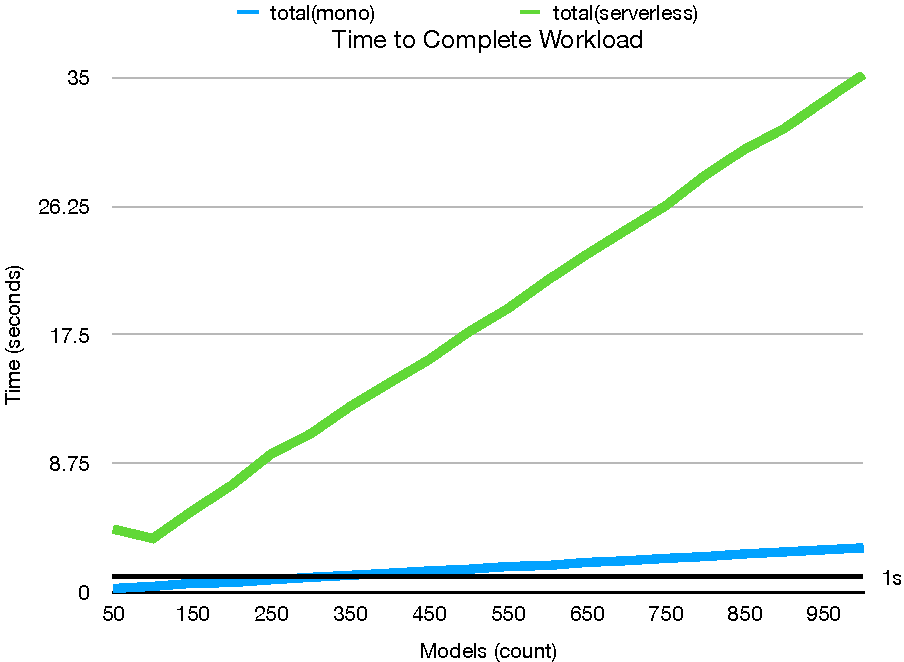
\includegraphics[width=\textwidth]{media/no_rl_ex.pdf}
    \caption{Execution time comparison between serverless and monolithic implementations}
    \label{fig:rate_unlimited_comparison}
\end{figure}
The serverless implementation's execution time increased incomparably to the monolithic version, as seen on figure 5.1.
While for both implementations the median latency did tend to increase, the serverless implementation's latency increased considerably faster, as seen in figures 5.2 and 5.3.
\begin{figure}[h!]
    \centering
    \begin{minipage}{0.48\textwidth}
        \centering
        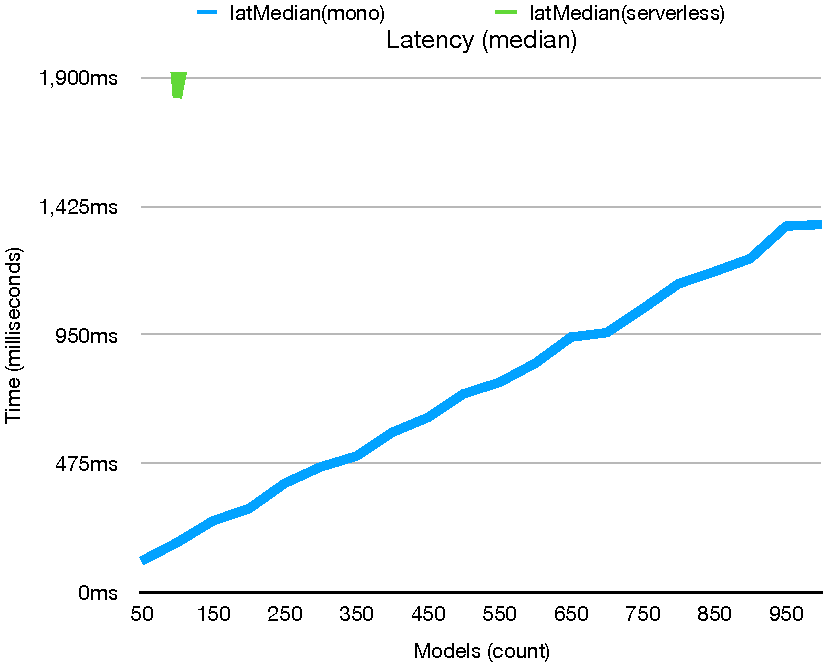
\includegraphics[width=\linewidth]{media/no_rl_mono_lat_med.pdf}
        \caption{Median latency for a single model request, scaled for the monolithic implementation}
        \label{fig:rate_unlimited_comparison_lat_mono}
    \end{minipage}\hfill
    \begin{minipage}{0.48\textwidth}
        \centering
        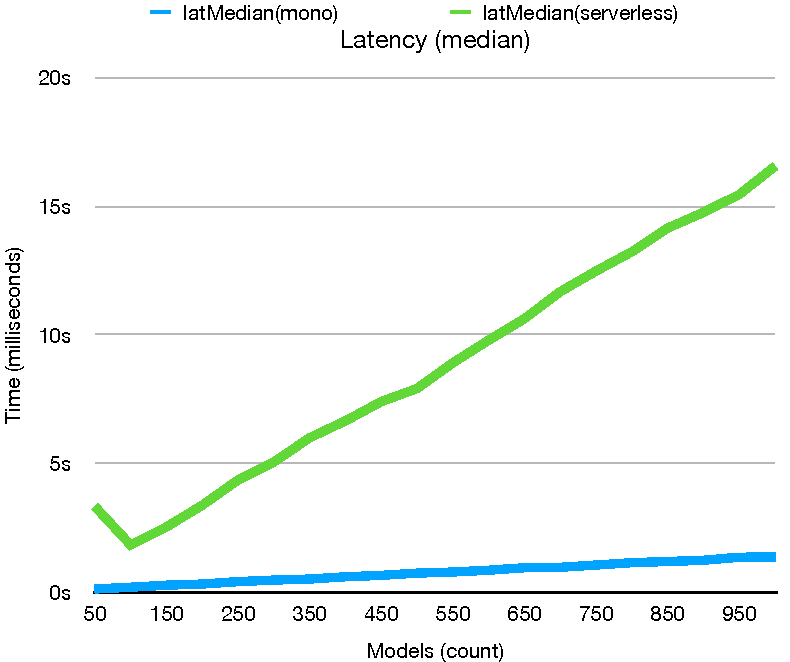
\includegraphics[width=\linewidth]{media/no_rl_lat_med.pdf}
        \caption{Median latency for a single model request}
        \label{fig:rate_unlimited_comparison_lat}
    \end{minipage}
\end{figure}

The above is explained by a much lower Queries per Second (QPS) by the serverless implementation. As seen on figure 5.4, while the serverless implementation seems to have hit a limit of 28 QPS, the serverless implementation seems to hit a limit of 333, more than ten times bigger.
\begin{figure}[h!]
    \centering
    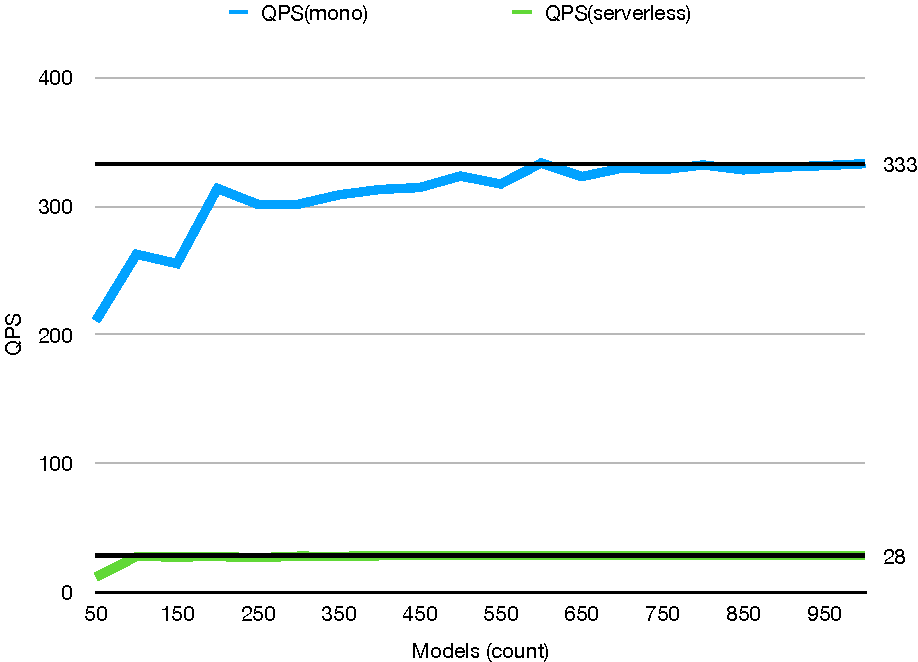
\includegraphics[width=\textwidth]{media/no_rl_qps.pdf}
    \caption{QPS comparison between serverless and monolithic implementations}
    \label{fig:rate_unlimited_comparison_qps}
\end{figure}


\subsection{Implementing a Rate Limit}
We use the Swift Rate Limitter, which is a custom made Swift rate limitter we have developed~\cite{swift-rl}, which is well tested, which allows us to send requests with a minimum set delay between them. We utilized it to send the requests every 100ms. This will cap the maximum QPS to 10 which ensures neither implementation will be stressed, hopefully allowing us to have a clearer picture of the situtation.

With the rate limit both implementations take the same amount of time and bot achieve roughly 10QPS.
As evident from figure 5.5, a single model sync takes roughly 280ms and 60ms on the serverless and monolithic implementations respectively.
\begin{figure}[h!]
    \centering
    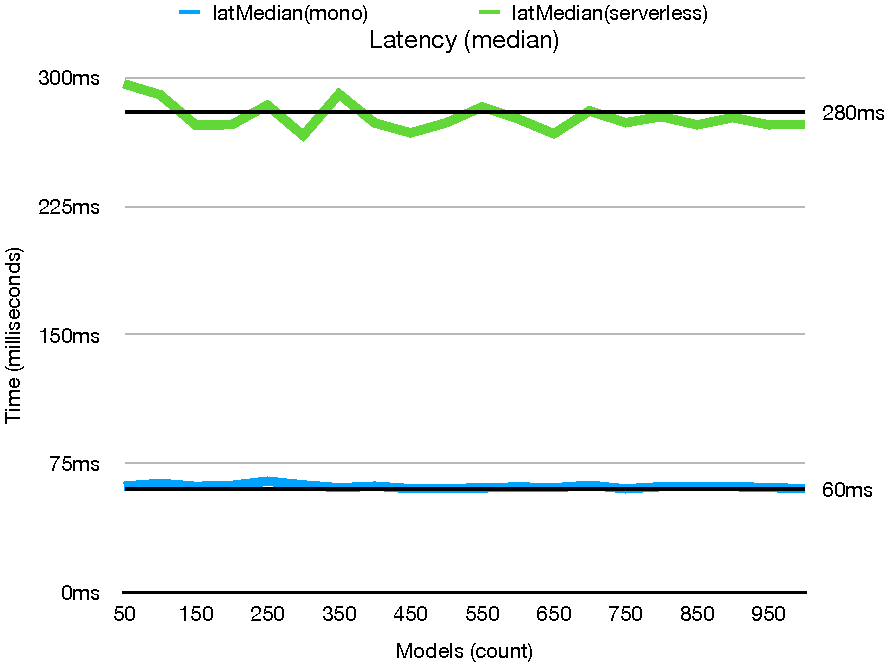
\includegraphics[width=\textwidth]{media/rl100_lat_med.pdf}
    \caption{Rate-limited (100ms) comparison between serverless and monolithic implementations}
    \label{fig:rate_limited_comparison}
\end{figure}
An interesting finding, is that the P99.9\% latency (figures 5.6 and 5.7), apart from being higher, it as less stable on the serverless implementation. This is despite utilizing less than the third of its maximum QPS.
\begin{figure}[h!]
    \centering
    \begin{minipage}{0.48\textwidth}
        \centering
        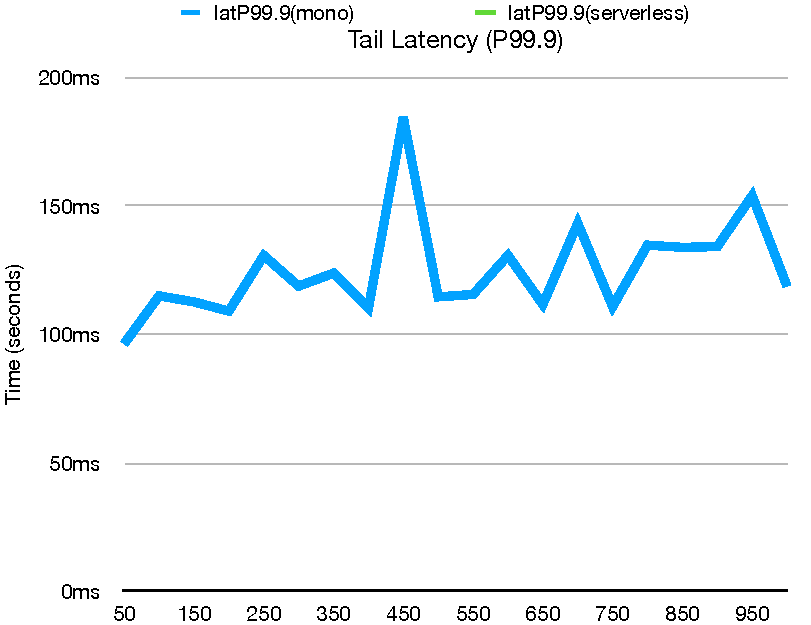
\includegraphics[width=\linewidth]{media/rl100_tl_mono.pdf}
        \caption{Median latency for a single model request, scaled for the monolithic implementation}
        \label{fig:rate_unlimited_comparison_lat_mono}
    \end{minipage}\hfill
    \begin{minipage}{0.48\textwidth}
        \centering
        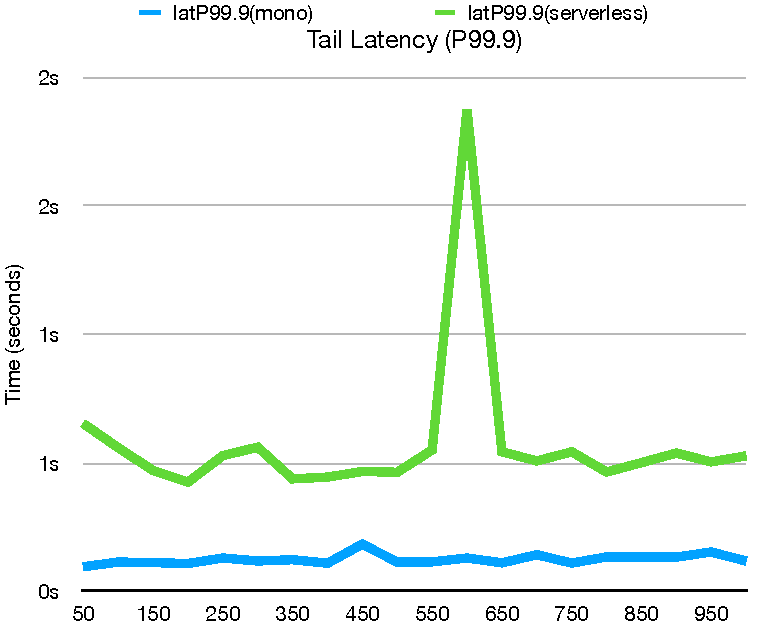
\includegraphics[width=\linewidth]{media/rl100_tl.pdf}
        \caption{Median latency for a single model request}
        \label{fig:rate_unlimited_comparison_lat}
    \end{minipage}
\end{figure}

Despite utilizing 18 machines for executing actions, the serverless approach did not show any clear benefits. This may be attributed to the lack of support for "intra-concurrency" in OpenWhisk runtimes, excluding NodeJS. This limitation significantly affects the scaling capabilities of the serverless implementation, which is a crucial aspect of the serverless or FaaS promise. 18 machines achieving 28QPS means that on average, a request takes 642ms to complete, which is more than double of the 280ms it takes, when the system is not stressed.

\section{Improvements and Future Work}

There are potential avenues for improvement in the serverless system. Notably, updating the Go proxy used by all OpenWhisk runtimes to support intra-concurrency could allow all language runtimes, including Swift, to support concurrent executions, potentially dramatically increasing the maximum QPS.

\section{Conclusion}

The case study findings contribute to the overall conclusion of this thesis, suggesting that the benefit of migrating to a serverless implementation is not always evident and should be carefully assessed for each workflow. The case study also highlights the importance of runtime support for intra-concurrency in realizing the full potential of serverless systems. Without intra-concurrency, the requests stay in memory until a container is available to serve them. The overheads of OpenWhisk may explain the 2 times slowdown of its request completion under load. Notably, the Swift runtime was updated to the latest version to leverage its native async/await features, which played a significant role in the serverless implementation. A total of eighteen identical machines achieving a throughput of ten times less than one single, identical machine is frankly unacceptable. Support for intra-concurrency for the ActionLoop proxy should be a priority for the OpenWhisk project as seamless, efficient scaling is the central promise of FaaS.


\chapter{Conclusion}
\label{chap:conclusion}
In concluding, it is evident that Swift holds substantial potential as a serverless language, albeit with several areas necessitating further development and exploration.

Swift's expressiveness and simplicity render it a productive choice for developers, offering a unique blend of performance and usability. However, a more comprehensive practical comparison with other serverless languages such as Python, JavaScript, or Go is imperative to fully comprehend its strengths and weaknesses in realistic serverless scenarios. This will not only validate Swift's theoretical advantages but also provide valuable insights for its future development.

One important aspect to consider, is that the decision to utilize serverless architecture should not be made lightly. While serverless computing offers scalability and reduces the need for server management, in some cases, a shift from a serverless to a monolithic architecture may lead to improved scalability, resilience, and cost-effectiveness, as was the case with the Prime Video service~\cite{primevideo2023}. This underscores the significance of a case-by-case analysis when deciding on the architectural choice, which is a subject of ongoing debate in the tech industry~\cite{virtualizationreview2023}.

The current state of Swift as a serverless language is promising, but there are limitations that need to be addressed. One of the key challenges is the lack of helpful feedback for some errors, which contradicts Swift's core promise of safety. Developers often find themselves needing to use \texttt{lldb} on remote machines to troubleshoot, which can be a significant hurdle in the development process.

Moreover, the need for better documentation and Linux support is evident. The absence of a built-in mechanism to ensure that all APIs used are supported on the Linux platform is a significant drawback. Developers are currently left to rely on Docker tests or discover at runtime if a feature is unsupported. Enhancing Linux support and providing comprehensive documentation would greatly improve Swift's fitness as a systems language and its viability as a serverless language.

In the context of OpenWhisk's ActionLoop proxy, the importance of intra-concurrency cannot be overstated. The case study results indicate that the lack of real concurrency wastes much of the hardware's potential and provides poor scaling, which is contrary to the essence of serverless. As most runtimes use the ActionLoop proxy, its support of concurrency is critically important for the efficient use of Swift in serverless settings.

Looking ahead, the future of Swift as a serverless language is bright, but it hinges on addressing these challenges and capitalizing on its strengths. The journey of Swift in the serverless landscape is just beginning, and with the right improvements, it can become a powerful tool in the hands of developers. In this journey, it is vital to remember that while serverless architecture offers many benefits, the decision between serverless and monolithic architectures should be made with careful consideration ofthe specific context and requirements of the project, as well illustrated by the case of Amazon's Prime Video service
%\chapter{Synchronization System Case Study}
\etocsettocstyle{\rule{\textwidth}{1pt}}{\rule{\textwidth}{1pt}} % style for toc
\localtableofcontents
\label{chap:synchronization}

In eCommerce, synchronization systems are often needed to ensure that the online store reflects the current state of the store's products' logistics. Brick-and-mortar stores manage their inventory with logistical software system. A synchronization system that ensures the consistency and truthfulness of the online store is crucial.
The main focus of this chapter is on a practical comparison between serverless and monolithic implementations of such a synchronization system. Synthetic workloads are generated and two mock servers, simulating a logistics system and a Shopify store are used.

\section{System Overview}
Suppose a brick-and-mortar store sells products. Each product has different variants. The store keeps track of its inventory with a logistics system. That system provides an API endpoint with which one can query data and modify it.
The store wishes to have an online eCommerce store. The platform of the store has an API endpoint for adding and modifying resources, such as the products.
A system is needed that ensures that the online store reflects the current state of the physical store. That means that Every product that exists on the physical store, should exist on the online store with the correct quantity. If a product sells out on the physical store, it is the job of the system to ensure that the lack of stock is present on the online store.
\subsection{Main Components}
PS will denote the server that runs the physical store's entrypoint.
SH will denote the server that runs the online store's endpoint. 
Syncer is the object that synchronizes a product between the two endpoints.





% bibliography
\bibliographystyle{abbrv}
\balance
\bibliography{thesis}


% that's all folks
\end{document}
